%!TEX program = xelatex
\documentclass[11pt, a4paper]{article}

% AA LINGUA E GESTIONE FONT (Specifica per XeLaTeX)
\usepackage{fontspec}
\setmainfont{Latin Modern Roman}
\usepackage[italian]{babel}

% AA LAYOUT DI PAGINA E TIPOGRAFIA (Ottimizzato per Rilegatura)
\usepackage[left=2.4cm, right=1.6cm, top=2cm, bottom=2cm]{geometry}

% AA Spaziatura tra paragrafi controllata (compatta ed evita salti enormi)
\usepackage[skip=3pt plus 1pt minus 1pt]{parskip}
\setlength{\parindent}{0pt}

% AA Microtype per XeLaTeX
\usepackage[protrusion=true]{microtype}
\raggedbottom

% AA GESTIONE DEI COLORI
\usepackage{xcolor}

% BB COLORI E MACRO PER I SIGMA
\definecolor{sigRed}{RGB}{215, 0, 0}
\definecolor{sigBlue}{RGB}{0, 70, 220}
\definecolor{sigGreen}{RGB}{0, 145, 45}

\newcommand{\sigA}{\textcolor{sigRed}{\boldsymbol{\sigma_A}}}
\newcommand{\sigB}{\textcolor{sigBlue}{\boldsymbol{\sigma_B}}}
\newcommand{\sigC}{\textcolor{sigGreen}{\boldsymbol{\sigma_C}}}

% AA MATEMATICA E SIMBOLI
\usepackage{amsmath}
\usepackage{mathtools}
\usepackage{silence}
\usepackage[warnings-off={mathtools-overbracket,mathtools-colon}]{unicode-math}
\setmathfont{Latin Modern Math}

% BB OTTIMIZZAZIONE MATRICI LUNGHE PER LA STAMPA
\setlength{\arraycolsep}{10pt}

% AA Spaziature verticali attorno alle formule matematiche
\setlength{\abovedisplayskip}{3pt plus 1pt minus 1pt}
\setlength{\belowdisplayskip}{3pt plus 1pt minus 1pt}
\setlength{\abovedisplayshortskip}{0pt plus 1pt}
\setlength{\belowdisplayshortskip}{2pt plus 1pt minus 1pt}

% AA GRAFICA ED IMMAGINI
\usepackage{graphicx}
\graphicspath{{./E8_Images/}}

% AA PERSONALIZZAZIONE TITOLI
\usepackage{titlesec}
\titleformat{\section}{\normalfont\Large\bfseries\color{blue!80!black}}{\thesection}{1em}{}
\titleformat{name=\section,numberless}{\normalfont\Large\bfseries\color{blue!80!black}}{}{0pt}{}

\titleformat{\subsection}{\normalfont\large\bfseries}{\thesubsection}{1em}{}
\titleformat{name=\subsection,numberless}{\normalfont\large\bfseries}{}{0pt}{}

\titleformat{\subsubsection}{\normalfont\normalsize\bfseries}{\thesubsubsection}{1em}{}
\titleformat{name=\subsubsection,numberless}{\normalfont\normalsize\bfseries}{}{0pt}{}

\titlespacing*{\section}{0pt}{1.2ex plus 0.4ex minus 0.2ex}{0.6ex plus 0.2ex}
\titlespacing*{\subsection}{0pt}{1ex plus 0.3ex minus 0.2ex}{0.5ex plus 0.2ex}
\titlespacing*{\subsubsection}{0pt}{0.8ex plus 0.2ex minus 0.1ex}{0.4ex plus 0.1ex}

\titleformat{\paragraph}[block]{\normalfont\normalsize\bfseries\color{black!80!black}\raggedright}{}{0pt}{}
\titlespacing*{\paragraph}{0pt}{1.2ex plus 0.3ex minus 0.2ex}{0.4ex}

% AA INTEGRAZIONE CODICE MATLAB
\usepackage{matlab}

% BB Riconfigurazione Automatica Titoli Esportati da MATLAB
\renewcommand{\matlabheading}[1]{\section*{#1}}
\renewcommand{\matlabheadingtwo}[1]{\subsection*{#1}}
\renewcommand{\matlabheadingthree}[1]{\subsubsection*{#1}}

% BB Formule E Matrici Simboliche
\renewenvironment{matlabsymbolicoutput}{%
  \par\vspace{2pt}%
  \begingroup
  \centering
}{%
  \par\vspace{2pt}%
  \endgroup
}

% BB Output Testuale Console
\renewenvironment{matlaboutput}{%
  \par\vspace{1pt}%
  \Verbatim[xleftmargin=10pt, formatcom=\color{black!75}, fontsize=\footnotesize]%
}{%
  \endVerbatim
  \vspace{1pt}%
}

% BB Box Codice (Stile Moderno con Barra Laterale Colorata)
\lstset{
  backgroundcolor={},
  aboveskip=0pt,
  belowskip=0pt,
  basicstyle=\ttfamily\footnotesize,
  xleftmargin=0pt
}

\mdfdefinestyle{matlabcode}{%
  topline=false,
  bottomline=false,
  rightline=false,
  leftline=true,
  linewidth=2.5pt,
  linecolor=blue!75!black,
  backgroundcolor=black!3,
  innertopmargin=4pt,
  innerbottommargin=4pt,
  innerleftmargin=9pt,
  innerrightmargin=6pt,
  skipabove=3pt,
  skipbelow=3pt
}

\allowdisplaybreaks

% AA LINK, METADATI ED ELENCHI
\usepackage{hyperref}
\hypersetup{
    colorlinks=true,
    linkcolor=blue!80!black,
    urlcolor=blue!80!black,
    citecolor=blue!80!black,
    pdftitle={Analisi Mobilità Manipolatore Planare RRR},
    pdfauthor={Francesco Lo Verde},
}
\usepackage{bookmark}

% BB Spaziatura Elenchi (Arieggiata per la Stampa)
\usepackage{enumitem}
\setlist{itemsep=3.5pt plus 1pt minus 1pt, topsep=4pt plus 1pt minus 1pt, partopsep=0pt, parsep=1pt}


\author{Francesco Lo Verde}
\begin{document}

\matlabtitle{Analisi Mobilità Manipolatore Planare RRR}

\begin{par}
\begin{flushleft}
L'analisi della mobilità istantanea di un manipolatore planare con tre giunti rotoidali (RRR) si basa sullo studio delle proprietà della matrice Jacobiana, $J(q)$, che lega le velocità dei giunti $\dot{q}$ alle velocità dell'end-effector $v$ tramite la relazione $v=J(q)\;\dot{q}$
\end{flushleft}
\end{par}

\begin{par}
\begin{flushleft}
Si devono determinare:
\end{flushleft}
\end{par}

\begin{itemize}
   \item{\begin{flushleft} Lo \textbf{Spazio} delle \textbf{Velocità Raggiungibili} ($R(J)$): L'insieme di tutte le velocità che l'end-effector può assumere. \end{flushleft}}
   \item{\begin{flushleft} Le \textbf{Direzioni} di \textbf{Moto Precluse} ($N(J^T )$): Le direzioni in cui l'end-effector non può muoversi istantaneamente. \end{flushleft}}
   \item{\begin{flushleft} Gli \textbf{Automovimenti} ($N(J)$): Le combinazioni di velocità dei giunti che non producono movimento dell'end-effector, ma solo un riarrangiamento interno del robot. \end{flushleft}}
\end{itemize}

\begin{matlabcode}
clc; clear; close all;
% Parametri Manipolatore
syms q1 q2 q3 l1 l2 l3 real;
\end{matlabcode}

\begin{par}
\begin{flushleft}
Il primo passo consiste nel definire matematicamente il robot e calcolare la posizione del suo end-effector utilizzando la convenzione di Denavit-Hartenberg (DH)
\end{flushleft}
\end{par}

\begin{matlabcode}
% Definizione Tabelle DH Struttura
DH_Table = [q1, 0, 0, l1;
            q2, 0, 0, l2;
            q3, 0, 0, l3];
% q1 = pi/4;
% q2 = pi/2;
% q3 = pi/4;

% Calcolo Matrici Trasformazione E Rotazione Struttura
[T, R] = Compute_DH_Transformations(DH_Table);

T00 = eye(4);
T01 = simplify(T(:,:,1));       % Trasformazione da 0 a 1
T02 = simplify(T01 * T(:,:,2)); % Trasformazione da 0 a 2
T03 = simplify(T02 * T(:,:,3)); % Trasformazione da 0 a 3
\end{matlabcode}

\begin{par}
\begin{flushleft}
Il vettore di posizione $p$ dell'end-effector può essere estratto dalla matrice $^0 T_3$ in quanto è la quarta colonna. Poiché l'analisi di mobilità si concentra sul piano $z$ si prendono le prime due componenti del vettore posizione.
\end{flushleft}
\end{par}

\begin{matlabcode}
% Posizione dell'End-Effector
p_E = T03(1:3, 4);
fprintf('Vettore Posizione p RRR Planare:');
disp(p_E);
\end{matlabcode}
\begin{matlaboutput}
Vettore Posizione p RRR Planare:
\end{matlaboutput}
\begin{matlabsymbolicoutput}
\hskip1em $\displaystyle \left(\begin{array}{c}
l_2 \,\cos \left(q_1 +q_2 \right)+l_1 \,\cos \left(q_1 \right)+l_3 \,\cos \left(q_1 +q_2 +q_3 \right)\\
l_2 \,\sin \left(q_1 +q_2 \right)+l_1 \,\sin \left(q_1 \right)+l_3 \,\sin \left(q_1 +q_2 +q_3 \right)\\
0
\end{array}\right)$
\end{matlabsymbolicoutput}

\newpage
\begin{par}
\begin{flushleft}
Lo \textbf{Jacobiano analitico}, indicato come $J_r (q)$, è la matrice che lega la velocità dei giunti $\dot{q}$ alla velocità lineare dell'end-effector $v$ secondo la relazione:
\end{flushleft}
\end{par}

\[
    v=J_r (q)\dot{q}
\]

\begin{par}
\begin{flushleft}
Dato che si conosce l'espressione simbolica del vettore posizione dell'end-effector $p$ in funzione del vettore delle coordinate dei giunti $q$, lo Jacobiano si calcola come la matrice delle derivate parziali di ogni componente della posizione rispetto a ogni coordinata di giunto.
\end{flushleft}
\end{par}

\[
    J_r (q) = \frac{\partial p}{\partial q}
\]

\vspace{1em}
\begin{matlabcode}
% Vettori z (Assi Di Rotazione)
z0 = T00(1:3, 3); % Asse di rotazione del giunto 1
z1 = T01(1:3, 3); % Asse di rotazione del giunto 2
z2 = T02(1:3, 3); % Asse di rotazione del giunto 3

% Vettori p (Posizioni Origini Dei Riferimenti)
p0 = T00(1:3, 4); % Origine del frame 0
p1 = T01(1:3, 4); % Origine del frame 1
p2 = T02(1:3, 4); % Origine del frame 2

% Valori Per J1
J_L1 = cross(z0, p_E - p0);
J_A1 = z0;
J1 = [J_L1; J_A1];

% Valori Per J2
J_L2 = cross(z1, p_E - p1);
J_A2 = z1;
J2 = [J_L2; J_A2];

% Valori Per J3
J_L3 = cross(z2, p_E - p2);
J_A3 = z2;
J3 = [J_L3; J_A3];

% Costruzione Jacobiano Geometrico
J_q = simplify([J1, J2, J3]);

fprintf('Jacobiano Geometrico Manipolatore RRR Planare Simbolico');
disp(J_q);
\end{matlabcode}
\begin{matlaboutput}
Jacobiano Geometrico Manipolatore RRR Planare Simbolico
\end{matlaboutput}
\begin{matlabsymbolicoutput}
\hskip1em $\displaystyle \begin{array}{l}
\left(\begin{array}{ccc}
-l_2 \,\sin \left(q_1 +q_2 \right)-l_1 \,\sin \left(q_1 \right)-\sigma_1  & -l_2 \,\sin \left(q_1 +q_2 \right)-\sigma_1  & -\sigma_1 \\
l_2 \,\cos \left(q_1 +q_2 \right)+l_1 \,\cos \left(q_1 \right)+\sigma_2  & l_2 \,\cos \left(q_1 +q_2 \right)+\sigma_2  & \sigma_2 \\
0 & 0 & 0\\
0 & 0 & 0\\
0 & 0 & 0\\
1 & 1 & 1
\end{array}\right)\\
\mathrm{}\\
\textrm{where}\\
\mathrm{}\\
\;\;\sigma_1 =l_3 \,\sin \left(q_1 +q_2 +q_3 \right)\\
\mathrm{}\\
\;\;\sigma_2 =l_3 \,\cos \left(q_1 +q_2 +q_3 \right)
\end{array}$
\end{matlabsymbolicoutput}
\begin{matlabcode}
% Estrazione Jacobiano Lineare (Prime Due Righe)
J_L = J_q(1:2,1:3);
fprintf('Jacobiano Lineare Manipolatore RRR Planare Simbolico:');
disp(J_L);
\end{matlabcode}
\begin{matlaboutput}
Jacobiano Lineare Manipolatore RRR Planare Simbolico:
\end{matlaboutput}
\begin{matlabsymbolicoutput}
\hskip1em $\displaystyle \begin{array}{l}
\left(\begin{array}{ccc}
-l_2 \,\sin \left(q_1 +q_2 \right)-l_1 \,\sin \left(q_1 \right)-\sigma_1  & -l_2 \,\sin \left(q_1 +q_2 \right)-\sigma_1  & -\sigma_1 \\
l_2 \,\cos \left(q_1 +q_2 \right)+l_1 \,\cos \left(q_1 \right)+\sigma_2  & l_2 \,\cos \left(q_1 +q_2 \right)+\sigma_2  & \sigma_2
\end{array}\right)\\
\mathrm{}\\
\textrm{where}\\
\mathrm{}\\
\;\;\sigma_1 =l_3 \,\sin \left(q_1 +q_2 +q_3 \right)\\
\mathrm{}\\
\;\;\sigma_2 =l_3 \,\cos \left(q_1 +q_2 +q_3 \right)
\end{array}$
\end{matlabsymbolicoutput}

\begin{par}
\begin{flushleft}
Una configurazione $q$ è \textbf{singolare} quando lo Jacobiano $J_r (q)$ perde di rango, ovvero $\rho \bigl(J_r (q)\bigr)<m$. Per una matrice non quadrata come in questo caso ($m\times n=2\times 3$).
\end{flushleft}
\end{par}

\begin{par}
\begin{flushleft}
Un metodo robusto per trovare queste condizioni è analizzare la matrice di Gram $J_r (q)\cdot {\bigl((J_r (q)\bigr)}^T$ che è sempre quadrata ($m\times m$) e perde di rango esattamente quando $J_r (q)$ perde di rango. La condizione di singolarità si traduce quindi nel trovare le configurazioni $q$ per cui il determinante di questa matrice è nullo.
\end{flushleft}
\end{par}

\begin{matlabcode}
% Calcolo Condizione Singolarità: det(J(q) * J(q)^T) = 0
G = J_L * J_L.';
det_G = simplify(det(G));

disp('Determinante Matrice Di Gram (det(J_r * J_r^T)):');
disp(det_G);
\end{matlabcode}
\begin{matlaboutput}
Determinante Matrice Di Gram (det(J_r * J_r^T)):
\end{matlaboutput}
\begin{matlabsymbolicoutput}
\hskip1em $\displaystyle \frac{{l_1 }^2 \,{l_2 }^2 }{2}+{l_1 }^2 \,{l_3 }^2 +{l_2 }^2 \,{l_3 }^2 -\frac{{l_1 }^2 \,{l_2 }^2 \,\cos \left(2\,q_2 \right)}{2}-{l_2 }^2 \,{l_3 }^2 \,\cos \left(2\,q_3 \right)-{l_1 }^2 \,{l_3 }^2 \,\cos \left(2\,q_2 +2\,q_3 \right)-l_1 \,l_2 \,{l_3 }^2 \,\cos \left(q_2 +2\,q_3 \right)-{l_1 }^2 \,l_2 \,l_3 \,\cos \left(2\,q_2 +q_3 \right)+l_1 \,l_2 \,{l_3 }^2 \,\cos \left(q_2 \right)+{l_1 }^2 \,l_2 \,l_3 \,\cos \left(q_3 \right)$
\end{matlabsymbolicoutput}
\begin{matlabcode}
assume(l1 > 0 & l2 > 0 & l3 > 0);
assume([q2, q3], 'real');

disp('Condizione Di Singolarità:');
disp(det_G == 0);
\end{matlabcode}
\begin{matlaboutput}
Condizione Di Singolarità:
\end{matlaboutput}
\begin{matlabsymbolicoutput}
\hskip1em $\displaystyle \frac{{l_1 }^2 \,{l_2 }^2 }{2}+{l_1 }^2 \,{l_3 }^2 +{l_2 }^2 \,{l_3 }^2 -\frac{{l_1 }^2 \,{l_2 }^2 \,\cos \left(2\,q_2 \right)}{2}-{l_2 }^2 \,{l_3 }^2 \,\cos \left(2\,q_3 \right)-{l_1 }^2 \,{l_3 }^2 \,\cos \left(2\,q_2 +2\,q_3 \right)-l_1 \,l_2 \,{l_3 }^2 \,\cos \left(q_2 +2\,q_3 \right)-{l_1 }^2 \,l_2 \,l_3 \,\cos \left(2\,q_2 +q_3 \right)+l_1 \,l_2 \,{l_3 }^2 \,\cos \left(q_2 \right)+{l_1 }^2 \,l_2 \,l_3 \,\cos \left(q_3 \right)=0$
\end{matlabsymbolicoutput}

\begin{par}
\begin{flushleft}
La \textit{condizione di singolarità} è complessa e difficile da interpretare direttamente. Spesso, le condizioni di singolarità dipendono dagli angoli relativi tra i bracci, non dalla loro orientazione globale. Per semplificare l'espressione, si considera il caso specifico in cui i bracci hanno lunghezza unitaria ($l_1 =l_2 =l_3 =1$) in modo da mantenere tutte le proprietà cinematiche rilevanti.
\end{flushleft}
\end{par}

\newpage
\begin{matlabcode}
% Sostituzione Parametri Lunghezza
det_G_Sub = subs(det_G, [l1, l2, l3], [1, 1, 1]);

% Semplificazione
det_G_Sub = simplify(det_G_Sub);

disp('Condizione Di Singolarità Semplificata Con l1=l2=l3=1:');
disp(det_G_Sub == 0);
\end{matlabcode}
\begin{matlaboutput}
Condizione Di Singolarità Semplificata Con l1=l2=l3=1:
\end{matlaboutput}
\begin{matlabsymbolicoutput}
\resizebox{\linewidth}{!}{%
$
\cos \left(q_2 \right)-\cos \left(2\,q_2 +q_3 \right)-\frac{\cos \left(2\,q_2 \right)}{2}-\cos \left(2\,q_3 \right)-\cos \left(2\,q_2 +2\,q_3 \right)-\cos \left(q_2 +2\,q_3 \right)+\cos \left(q_3 \right)+\frac{5}{2}=0
$}
\end{matlabsymbolicoutput}

\begin{par}
\begin{flushleft}
La condizione di singolarità semplificata ottenuta per lunghezze unitarie rivela che le singolarità dipendono solo dagli angoli $q_2$ e $q_3$. Questo è coerente con la natura planare del manipolatore, dove la posa della base non altera la raggiungibilità dello spazio di lavoro ma solo la sua orientazione. Le condizioni esatte in cui il determinante si annulla corrispondono a configurazioni geometricamente significative:
\end{flushleft}
\end{par}

\begin{itemize}

   \item{\begin{flushleft} Quando i bracci sono completamente estesi o ripiegati, l'end-effector si trova sul confine dello spazio di lavoro e perde un grado di libertà (\textit{Singolarità Di Bordo}). Questo accade quando $q_2$ 0 $q_3$ sono $0$ oppure $\pi$. \end{flushleft}}
   \item{\begin{flushleft} Quando l'end-effector si ripiega su un giunto precedente, cioè la punta del robot si trova alla base del giunto $q_1$. Questa singolarità dipende dalle lunghezze dei bracci e dagli angoli $q_2$ e $q_3$. \end{flushleft}}
\end{itemize}

\begin{par}
\begin{flushleft}
Quindi, poichè la matrice Jacobiana $J$ non è costante, ma dipende dalla configurazione attuale del robot, descritta dal vettore delle variabili di giunto, il determinante e tutte le proprietà (rango, immagine e nucleo) sono \textbf{locali}, ovvero variano con $q$:
\end{flushleft}
\end{par}
\[
    det(J)=det(J(q)) \qquad \rho (J)=\rho J(q) \qquad R(J)=R(J(q)) \qquad N(J)=N(J(q))
\]



\vspace{1em}
\matlabheadingtwo{Configurazione 1: Robot Ripiegato}

\begin{par}
\begin{flushleft}
I parametri del robot sono
\end{flushleft}
\end{par}

\begin{par}
$$l_1 =l_2 =l_3 =1$$
\end{par}

\begin{par}
$$q_1 =0~~~~q_2 =\frac{\pi }{2}~~~~q_3 =-\frac{\pi }{2}$$
\end{par}


\vspace{1em}
\begin{matlabcode}
% Valori numerici per la configurazione
l_vals = [1, 1, 1];
q1_val = 0;
q2_val = pi/2;
q3_val = -pi/2;
q_vals = [q1_val, q2_val, q3_val];

fprintf('------------ Configurazione q = [%.2f, %.2f, %.2f] ------------', q_vals(1), q_vals(2), q_vals(3));
\end{matlabcode}
\begin{matlaboutput}
--------------- Configurazione q = [0.00, 1.57, -1.57] ---------------
\end{matlaboutput}
\newpage
\begin{matlabcode}

% Sostituzione dei valori numerici nello Jacobiano lineare simbolico
vars_sym = [l1, l2, l3, q1, q2, q3];
vals_num = [l_vals, q_vals];
J1_num = double(subs(J_L, vars_sym, vals_num));

fprintf('Jacobiano Lineare Numerico:\n');
disp(J1_num);
\end{matlabcode}
\begin{matlaboutput}
Jacobiano Lineare Numerico:
\end{matlaboutput}

\begin{matlaboutput}
    -1    -1     0
     2     1     1
\end{matlaboutput}
\begin{matlabcode}
% Verifica Singolarità
rank_J1 = rank(J1_num);
fprintf('Rango dello Jacobiano: %d\n', rank_J1);
\end{matlabcode}
\begin{matlaboutput}
Rango dello Jacobiano: 2
\end{matlaboutput}
\begin{matlabcode}
% Dimensione Spazio Lavoro
m = size(J_L, 1);
% Numero Di Giunti
n = size(DH_Table, 1);

if rank_J1 < m
    fprintf('Configurazione Singolare (Rango < m)');

    % Spazio Velocità Raggiungibili (Immagine di J)
    R_J1 = orth(J1_num);
    fprintf('Base Spazio Velocità Raggiungibili R(J):\n');
    disp(R_J1);
    % L'End-Effector Può Muoversi Solo Lungo La Direzione Di Questo Vettore

    % Direzioni Di Moto Precluse (Nucleo di J^T)
    N_J1_T = null(J1_num.');
    fprintf('Base Direzioni Di Moto Precluse N(J^T):\n');
    disp(N_J1_T);
    % L'End-Effector È Bloccato E Non Può Muoversi Lungo Direzione Di Questo Vettore
else
    fprintf('Configurazione NON Singolare (Rango Pieno)');

    % Spazio Velocità Raggiungibili (Immagine di J)
    R_J1 = orth(J1_num);
    fprintf('Base Spazio Velocità Raggiungibili R(J):\n');
    disp(R_J1);
    % L'End-Effector Può Muoversi Solo Lungo La Direzione Di Questo Vettore

    % Direzioni Di Moto Precluse (Nucleo di J^T)
    fprintf('Non Ci Sono Direzioni Di Moto Precluse N(J^T)!');
end
\end{matlabcode}
\begin{matlaboutput}
Configurazione NON Singolare (Rango Pieno)
Base Spazio Velocità Raggiungibili R(J):
    0.4719    0.8817
   -0.8817    0.4719
Non Ci Sono Direzioni Di Moto Precluse N(J^T)!
\end{matlaboutput}
\newpage
\begin{matlabcode}

% Per Robot Ridondanti
if n > m
    % Automovimenti (Nucleo di J)
    A_J1 = null(J1_num);
    fprintf('Base Automovimenti N(J):\n');
    disp(A_J1);
    % Sono Possibili Due Moti Senza Spostare La Punta Del Robot
    dim_A = size(A_J1, 2);
    fprintf('Numero Automovimenti: %d', dim_A);
else
    fprintf('Robot Non Ridondante (n <= m), Non Esistono Automovimenti');
end
\end{matlabcode}
\begin{matlaboutput}
Base Automovimenti N(J):
   -0.5774
    0.5774
    0.5774
Numero Automovimenti: 1
\end{matlaboutput}

\matlabheadingthree{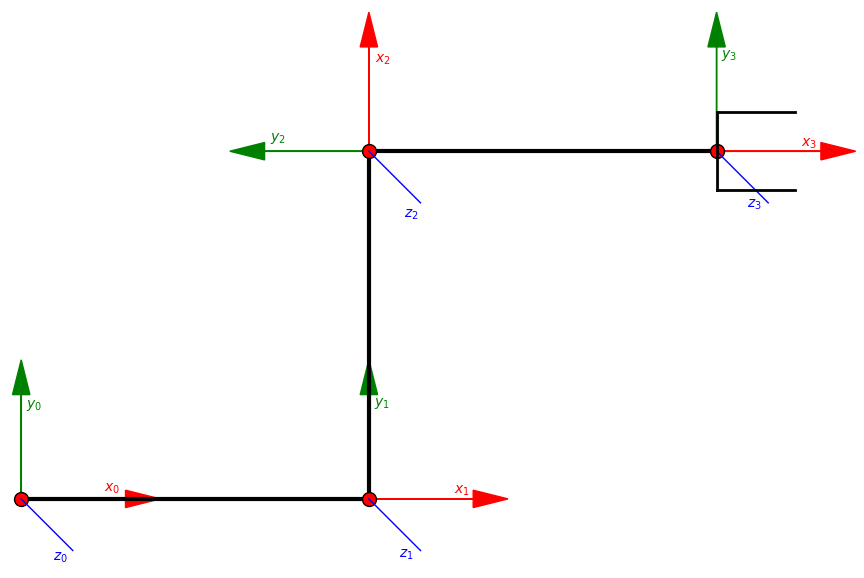
\includegraphics[width=0.75\linewidth]{image_0}}

\matlabheadingthree{\textbf{Giustificazione Risultati Punto Di Vista Meccanico}}

\begin{par}
\begin{flushleft}
In questa configurazione:
\begin{enumerate}
   \item \begin{flushleft} Il primo braccio $l_1$ giace lungo l'asse X, poiché $q_1=0$. \end{flushleft}
   \item \begin{flushleft} Il secondo braccio $l_2$ è ruotato di $q_2 = \frac{\pi}{2}$ rispetto al primo, puntando quindi lungo l'asse Y. \end{flushleft}
   \item \begin{flushleft} Il terzo braccio $l_3$ è ruotato di $q_3 = \frac{\pi}{2}$ rispetto al secondo, risultando quindi parallelo all'asse X e orientato nella stessa direzione del primo braccio. \end{flushleft}
   \item \begin{flushleft} La posizione dell'end-effector è la somma vettoriale dei bracci: $p_E = (l_1 + l_3, l_2) = (1+0, 1) = (1,1)$. \end{flushleft}
\end{enumerate}

\end{flushleft}
\end{par}
\newpage

\begin{par}
\begin{flushleft}
\textbf{Analisi di Mobilità \textit{(Configurazione NON Singolare)}}
\end{flushleft}
\end{par}

\begin{par}
\begin{flushleft}
Il calcolo mostra che il \textbf{rango} dello \textbf{Jacobiano} è \textbf{2}, ovvero il massimo possibile (rango pieno), dato che lo spazio di lavoro è bidimensionale ($m=2$).

Poiché $\rho(J_L)=m$, lo Spazio delle Velocità Raggiungibili $R(J_L)$ coincide con l'intero piano $\mathbb{R}^2$. Di conseguenza, il suo complemento ortogonale, lo spazio delle Direzioni di Moto Precluse $N(J_L^T)$, è banale (contiene solo il vettore nullo).

La configurazione non è singolare perché i movimenti generati dai singoli giunti sono linearmente indipendenti. Una rotazione del giunto 1 ($\dot{q}_1$) farebbe ruotare l'intera struttura attorno all'origine, producendo una velocità dell'end-effector istantaneamente tangente a un cerchio (in questo caso, lungo la direzione $[-1,1]$). Le rotazioni dei giunti 2 e 3 ($\dot{q}_2, \dot{q}_3$) producono movimenti che non sono paralleli a quello generato dal giunto 1. Poiché è possibile generare velocità in direzioni non collineari, la loro combinazione lineare può produrre un vettore di velocità arbitrario nel piano $(v_x, v_y)$. L'end-effector può quindi muoversi istantaneamente in qualsiasi direzione.
\end{flushleft}
\end{par}

\begin{par}
\begin{flushleft}
\textbf{Analisi degli Automovimenti \textit{(Ridondanza)}}
\end{flushleft}
\end{par}

\begin{par}
\begin{flushleft}
Il manipolatore è ridondante per il posizionamento 2D ($n=3>m=2$). La dimensione dello spazio nullo (automovimenti) è data da
$n - \rho(J_L) = 3 - 2 = 1$.

Esiste una base per $N(J_L)$ con un solo vettore, come calcolato. Questo vettore definisce una combinazione specifica di velocità dei giunti $\dot{q} \in N(J_L)$ che risulta in una velocità nulla dell'end-effector $v = J_L \dot{q} = 0$.

La presenza di un automovimento significa che il robot può \textbf{riconfigurare la sua postura interna mantenendo l'end-effector fermo}. Si può immaginare un movimento coordinato del giunto 2 e del giunto 3, compensato dal giunto di base (giunto 1), che permette alla struttura di muoversi pur mantenendo la punta fissa in $(1,1)$. Questa capacità aggiuntiva è un vantaggio della ridondanza, utilizzata ad esempio per evitare ostacoli con il corpo del robot senza spostare l'end-effector.
\end{flushleft}
\end{par}

\vspace{1em}

\matlabheadingtwo{Configurazione 2: Robot Completamente Esteso}

\begin{par}
\begin{flushleft}
I parametri del robot sono
\end{flushleft}
\end{par}

\begin{par}
$$l_1 =l_2 =l_3 =1$$
\end{par}

\begin{par}
$$q_1 =0~~~~q_2 =\pi ~~~~q_3 =0$$
\end{par}

\begin{matlabcode}
% Valori numerici per la configurazione
q1_val_2 = 0;
q2_val_2 = pi;
q3_val_2 = 0;
q_vals_2 = [q1_val_2, q2_val_2, q3_val_2];

fprintf('------------ Configurazione q = [%.2f, %.2f, %.2f] ------------', q_vals_2(1), q_vals_2(2), q_vals_2(3));

% Sostituzione dei valori numerici nello Jacobiano lineare simbolico
vars_sym = [l1, l2, l3, q1, q2, q3];
vals_num = [l_vals, q_vals_2];
J1_num = double(subs(J_L, vars_sym, vals_num));

fprintf('Jacobiano Lineare Numerico:\n');
disp(J1_num);
\end{matlabcode}
\begin{matlaboutput}
------------ Configurazione q = [0.00, 3.14, 0.00] ------------
Jacobiano Lineare Numerico:
     0     0     0
    -1    -2    -1
\end{matlaboutput}
\begin{matlabcode}
% Verifica Singolarità
rank_J1 = rank(J1_num);
fprintf('Rango dello Jacobiano: %d\n', rank_J1);
\end{matlabcode}
\begin{matlaboutput}
Rango dello Jacobiano: 1
\end{matlaboutput}
\begin{matlabcode}

% Dimensione Spazio Lavoro
m = size(J_L, 1);
% Numero Di Giunti
n = size(DH_Table, 1);

if rank_J1 < m
    fprintf('Configurazione Singolare (Rango < m)');

    % Spazio Velocità Raggiungibili (Immagine di J)
    R_J1 = orth(J1_num);
    fprintf('Base Spazio Velocità Raggiungibili R(J):\n');
    disp(R_J1);
    % L'End-Effector Può Muoversi Solo Lungo La Direzione Di Questo Vettore

    % Direzioni Di Moto Precluse (Nucleo di J^T)
    N_J1_T = null(J1_num.');
    fprintf('Base Direzioni Di Moto Precluse N(J^T):\n');
    disp(N_J1_T);
    % L'End-Effector È Bloccato E Non Può Muoversi Lungo Direzione Di Questo Vettore
else
    fprintf('Configurazione NON Singolare (Rango Pieno)');

    % Spazio Velocità Raggiungibili (Immagine di J)
    R_J1 = orth(J1_num);
    fprintf('Base Spazio Velocità Raggiungibili R(J):\n');
    disp(R_J1);
    % L'End-Effector Può Muoversi Solo Lungo La Direzione Di Questo Vettore

    % Direzioni Di Moto Precluse (Nucleo di J^T)
    fprintf('Non Ci Sono Direzioni Di Moto Precluse N(J^T)!');
end
\end{matlabcode}
\begin{matlaboutput}
Configurazione Singolare (Rango < m)
Base Spazio Velocità Raggiungibili R(J):
     0
     1
Base Direzioni Di Moto Precluse N(J^T):
    -1
     0
\end{matlaboutput}
\newpage
\begin{matlabcode}
% Per Robot Ridondanti
if n > m
    % Automovimenti (Nucleo di J)
    A_J1 = null(J1_num);
    fprintf('Base Automovimenti N(J):\n');
    disp(A_J1);
    % Sono Possibili Due Moti Senza Spostare La Punta Del Robot
    dim_A = size(A_J1, 2);
    fprintf('Numero Automovimenti: %d', dim_A);
else
    fprintf('Robot Non Ridondante (n <= m), Non Esistono Automovimenti');
end
\end{matlabcode}
\begin{matlaboutput}
Base Automovimenti N(J):
   -0.9129         0
    0.3651   -0.4472
    0.1826    0.8944
Numero Automovimenti: 2
\end{matlaboutput}

\matlabheadingthree{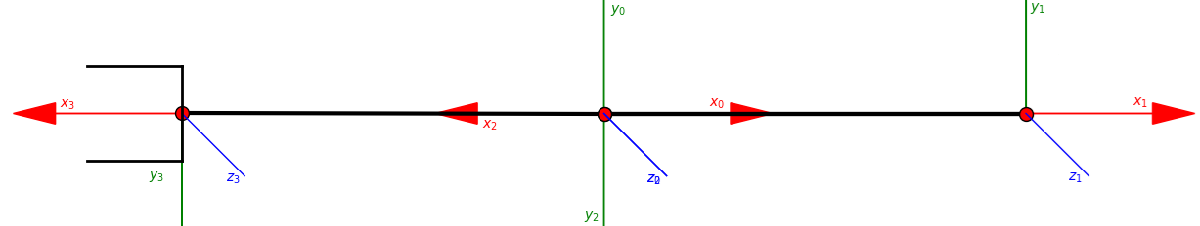
\includegraphics[width=0.85\linewidth]{image_1}}

\matlabheadingthree{\texttt{\textbf{Giustificazione Risultati Punto Di Vista Meccanico}}}

\begin{par}
\begin{flushleft}
In questa configurazione, il robot è ripiegato su se stesso:
\begin{enumerate}
   \item \begin{flushleft} Il primo braccio $l_1$ è orientato lungo l'asse X ($q_1 = 0$). \end{flushleft}
    \item \begin{flushleft} Il secondo braccio $l_2$ è ruotato di $q_2 = \pi$, ripiegandosi completamente all'indietro e allineandosi con l'asse X in direzione negativa. \end{flushleft}
    \item \begin{flushleft} Il terzo braccio $l_3$ è ruotato di $q_3 = 0$ rispetto al secondo, quindi prosegue nella stessa direzione del secondo braccio. \end{flushleft}
    \item \begin{flushleft} La posizione dell'end-effector è $p_E = (-1,0)$. \end{flushleft}
\end{enumerate}
\end{flushleft}
\end{par}

\begin{par}
\begin{flushleft}
\textbf{Analisi di Mobilità \textit{(Configurazione Singolare)}}
\end{flushleft}
\end{par}

\begin{par}
\begin{flushleft}
Il calcolo mostra che il \textbf{rango} dello \textbf{Jacobiano} è \textbf{1}. Poiché $\rho(J_L)<m$, la configurazione è \textbf{singolare}.

Lo Spazio delle Velocità Raggiungibili $R(J_L)$ ha dimensione 1. La sua base, data dal vettore $[0,1]^T$, indica che l'unica direzione di moto possibile è lungo l'asse Y. Le Direzioni di Moto Precluse $N(J_L^T)$ hanno dimensione $m - \rho(J_L) = 2-1 = 1$. La sua base, data dal vettore $[-1,0]^T$, indica che il moto lungo l'asse X è impossibile.

La singolarità emerge perché tutti i bracci sono allineati. Qualsiasi piccola rotazione di uno qualsiasi dei tre giunti provoca un movimento della punta del robot, che in questa postura è sempre perpendicolare alla linea dei bracci (cioè, lungo l'asse Y). È fisicamente impossibile generare una velocità istantanea dell'end-effector lungo la direzione dei bracci stessi (l'asse X). Un tentativo di spingere o tirare l'end-effector lungo l'asse X si tradurrebbe solo in forze di compressione/trazione interne alla struttura, senza produrre alcun movimento.
\end{flushleft}
\end{par}

\begin{par}
\begin{flushleft}
\textbf{Analisi degli Automovimenti \textit{(Effetto Singolarità)}}
\end{flushleft}
\end{par}

\begin{par}
\begin{flushleft}
In una configurazione singolare, la dimensione dello spazio degli automovimenti aumenta, cioè $n - \rho(J_L) = 3-1 = 2$.

Esistono due combinazioni linearmente indipendenti di velocità dei giunti che mantengono l'end-effector fermo. La base di $N(J_L)$ calcolata contiene i due vettori che definiscono questi movimenti. La perdita di un grado di libertà nel movimento dell'end-effector (non può muoversi lungo l'asse X) si traduce in un \textbf{guadagno di un grado di libertà nel movimento} del robot. Oltre all'automovimento già presente dovuto alla ridondanza, la singolarità ne introduce un secondo. Intuitivamente, i giunti possono muoversi in modi più complessi e coordinati (descritti dai due vettori) per riarrangiare la postura del robot lungo l'asse X senza che la punta, bloccata a $x=-1$, si sposti.
\end{flushleft}
\end{par}





\end{document}
